% !TeX spellcheck = pl_PL
%%%%%%%%%%%%%%%%%%%%%%%%%%%%%%%%%%%%%%%%%%%
%                                        %
% Szablon pracy dyplomowej inzynierskiej %
% zgodny  z aktualnymi  przepisami  SZJK %
%                                        %
%%%%%%%%%%%%%%%%%%%%%%%%%%%%%%%%%%%%%%%%%%
%                                        %
%  (c) Krzysztof Simiński, 2018-2023     %
%                                        %
%%%%%%%%%%%%%%%%%%%%%%%%%%%%%%%%%%%%%%%%%%
%                                        %
% Najnowsza wersja szablonów jest        %
% podstępna pod adresem                  %
% github.com/ksiminski/polsl-aei-theses  %
%                                        %
%%%%%%%%%%%%%%%%%%%%%%%%%%%%%%%%%%%%%%%%%%
%
%
% Projekt LaTeXowy zapewnia odpowiednie formatowanie pracy,
% zgodnie z wymaganiami Systemu zapewniania jakości kształcenia.
% Proszę nie zmieniać ustawień formatowania (np. fontu,
% marginesów, wytłuszczeń, kursywy itd. ).
%
% Projekt można kompilować na kilka sposobów.
%
% 1. kompilacja pdfLaTeX
%
% pdflatex main
% bibtex   main
% pdflatex main
% pdflatex main
%
%
% 2. kompilacja XeLaTeX
%
% Kompilatacja przy użyciu XeLaTeXa różni się tym, że na stronie
% tytułowej używany jest font Calibri. Wymaga to jego uprzedniego
% zainstalowania.
%
% xelatex main
% bibtex  main
% xelatex main
% xelatex main
%
%
%%%%%%%%%%%%%%%%%%%%%%%%%%%%%%%%%%%%%%%%%%%%%%%%%%%%%
% W przypadku pytań, uwag, proszę pisać na adres:   %
%      krzysztof.siminski(małpa)polsl.pl            %
%%%%%%%%%%%%%%%%%%%%%%%%%%%%%%%%%%%%%%%%%%%%%%%%%%%%%
%
% Chcemy ulepszać szablony LaTeXowe prac dyplomowych.
% Wypełniając ankietę spod poniższego adresu pomogą
% Państwo nam to zrobić. Ankieta jest całkowicie
% anonimowa. Dziękujemy!


% https://docs.google.com/forms/d/e/1FAIpQLScyllVxNKzKFHfILDfdbwC-jvT8YL0RSTFs-s27UGw9CKn-fQ/viewform?usp=sf_link
%
%%%%%%%%%%%%%%%%%%%%%%%%%%%%%%%%%%%%%%%%%%%%%%%%%%%%%%%%%%%%%%%%%%%%%%%%%

%%%%%%%%%%%%%%%%%%%%%%%%%%%%%%%%%%%%%%%%%%%%%%%
%                                             %
% PERSONALIZACJA PRACY – DANE PRACY           %
%                                             %
%%%%%%%%%%%%%%%%%%%%%%%%%%%%%%%%%%%%%%%%%%%%%%%

% Proszę wpisać swoje dane w poniższych definicjach.

% TODO
% dane autora
\newcommand{\FirstNameAuthor}{Michał}
\newcommand{\SurnameAuthor}{Lubczyński}
\newcommand{\IdAuthor}{}   % numer albumu  (bez $\langle$ i $\rangle$)

% drugi autor:
%\newcommand{\FirstNameCoauthor}{Imię}   % Jeżeli jest drugi autor, to tutaj należy podać imię.
%\newcommand{\SurnameCoauthor}{Nazwisko} % Jeżeli jest drugi autor, to tutaj należy podać nazwisko.
%\newcommand{\IdCoauthor}{$\langle$wpisać właściwy$\rangle$}  % numer albumu drugiego autora (bez $\langle$ i $\rangle$)
% Gdy nie ma drugiego autora, należy zostawić poniższe definicje puste, jak poniżej. Gdy jest drugi autor, należy zakomentować te linie.
\newcommand{\FirstNameCoauthor}{Andrzej} % Jeżeli praca ma tylko jednego autora, to dane drugiego autora zostają puste.
\newcommand{\SurnameCoauthor}{Zagórski}   % Jeżeli praca ma tylko jednego autora, to dane drugiego autora zostają puste.
\newcommand{\IdCoauthor}{}  % Jeżeli praca ma tylko jednego autora, to dane drugiego autora zostają puste.
%%%%%%%%%%
\newcommand{\FirstNameCoXauthor}{Eryk} % Jeżeli praca ma tylko jednego autora, to dane drugiego autora zostają puste.
\newcommand{\SurnameCoXauthor}{SZMYT}   % Jeżeli praca ma tylko jednego autora, to dane drugiego autora zostają puste.
\newcommand{\IdCoCoauthor}{}  % Jeżeli praca ma tylko jednego autora, to dane drugiego autora zostają puste.

\newcommand{\Supervisor}{Dr. Inż. Aleksander Iwaniak}     % dane promotora (bez $\langle$ i $\rangle$)
\newcommand{\Title}{Framer - Wizualizacja danych z kamery termowizyjnej}           % tytuł pracy po polsku
\newcommand{\TitleAlt}{Framer - Thermal Camera Data Visualizatioh}                     % thesis title in English
\newcommand{\Program}{}            % kierunek studiów  (bez $\langle$ i $\rangle$)
\newcommand{\Specialisation}{}     % specjalność  (bez $\langle$ i $\rangle$)
\newcommand{\Departament}{}        % katedra promotora  (bez $\langle$ i $\rangle$)

% Jeżeli został wyznaczony promotor pomocniczy lub opiekun, proszę go/ją wpisać ...
\newcommand{\Consultant}{} % dane promotora pomocniczego, opiekuna (bez $\langle$ i $\rangle$)
% ... w przeciwnym razie proszę zostawić puste miejsce jak poniżej:
%\newcommand{\Consultant}{} % brak promotowa pomocniczego / opiekuna

% koniec fragmentu do modyfikacji
%%%%%%%%%%%%%%%%%%%%%%%%%%%%%%%%%%%%%%%%%%


%%%%%%%%%%%%%%%%%%%%%%%%%%%%%%%%%%%%%%%%%%%%%%%
%                                             %
% KONIEC PERSONALIZACJI PRACY                 %
%                                             %
%%%%%%%%%%%%%%%%%%%%%%%%%%%%%%%%%%%%%%%%%%%%%%%

%%%%%%%%%%%%%%%%%%%%%%%%%%%%%%%%%%%%%%%%


%%%%%%%%%%%%%%%%%%%%%%%%%%%%%%%%%%%%%%%%%%%%%%%
%                                             %
% PROSZĘ NIE MODYFIKOWAĆ PONIŻSZYCH USTAWIEŃ! %
%                                             %
%%%%%%%%%%%%%%%%%%%%%%%%%%%%%%%%%%%%%%%%%%%%%%%



\documentclass[a4paper,twoside,12pt]{book}
\usepackage[utf8]{inputenc}                                      
\usepackage[T1]{fontenc}  
\usepackage{amsmath,amsfonts,amssymb,amsthm}
\usepackage[british,polish]{babel} 
\usepackage{indentfirst}
\usepackage{xurl}
\usepackage{xstring}
\usepackage{ifthen}
\usepackage{graphicx}
\usepackage{float}



\usepackage{ifxetex}

\ifxetex
	\usepackage{fontspec}
	\defaultfontfeatures{Mapping=tex—text} % to support TeX conventions like ``——-''
	\usepackage{xunicode} % Unicode support for LaTeX character names (accents, European chars, etc)
	\usepackage{xltxtra} % Extra customizations for XeLaTeX
\else
	\usepackage{lmodern}
\fi



\usepackage[margin=2.5cm]{geometry}
\usepackage{hyperref}
\usepackage{booktabs}
\usepackage{tikz}
\usepackage{pgfplots}
\usepackage{mathtools}
\usepackage{geometry}
\usepackage{subcaption}   % subfigures
\usepackage[page]{appendix} % toc,
\renewcommand{\appendixtocname}{Dodatki}
\renewcommand{\appendixpagename}{Dodatki}
\renewcommand{\appendixname}{Dodatek}

\usepackage{csquotes}
\usepackage[natbib=true,backend=bibtex,maxbibnames=99]{biblatex}  % kompilacja bibliografii BibTeXem
%\usepackage[natbib=true,backend=biber,maxbibnames=99]{biblatex}  % kompilacja bibliografii Biberem
\bibliography{biblio}

\usepackage{ifmtarg}   % empty commands  

\usepackage{setspace}
\onehalfspacing


\frenchspacing



%%%% TODO LIST GENERATOR %%%%%%%%%

\usepackage{color}
\definecolor{brickred}      {cmyk}{0   , 0.89, 0.94, 0.28}

\makeatletter \newcommand \kslistofremarks{\section*{Uwagi} \@starttoc{rks}}
  \newcommand\l@uwagas[2]
    {\par\noindent \textbf{#2:} %\parbox{10cm}
{#1}\par} \makeatother


\newcommand{\ksremark}[1]{%
{%\marginpar{\textdbend}
{\color{brickred}{[#1]}}}%
\addcontentsline{rks}{uwagas}{\protect{#1}}%
}

\newcommand{\comma}{\ksremark{przecinek}}
\newcommand{\nocomma}{\ksremark{bez przecinka}}
\newcommand{\styl}{\ksremark{styl}}
\newcommand{\ortografia}{\ksremark{ortografia}}
\newcommand{\fleksja}{\ksremark{fleksja}}
\newcommand{\pauza}{\ksremark{pauza `--', nie dywiz `-'}}
\newcommand{\kolokwializm}{\ksremark{kolokwializm}}
\newcommand{\cudzyslowy}{\ksremark{,,polskie cudzysłowy''}}

%%%%%%%%%%%%%% END OF TODO LIST GENERATOR %%%%%%%%%%%

\newcommand{\printCoauthor}{%		
    \StrLen{\FirstNameCoauthor}[\FNCoALen]
    \ifthenelse{\FNCoALen > 0}%
    {%
		{\large\bfseries\Coauthor\par}
	
		{\normalsize\bfseries \LeftId \IdCoauthor\par}
		\vspace{2mm}

		{\large\bfseries\FirstNameCoXauthor\space \SurnameCoXauthor}
	

    }%
    {}
} 

%%%%%%%%%%%%%%%%%%%%%
\newcommand{\autor}{%		
    \StrLen{\FirstNameCoauthor}[\FNCoALenXX]
    \ifthenelse{\FNCoALenXX > 0}%
    {\Title}%
	{\FirstNameAuthor\ \SurnameAuthor}%
}
%%%%%%%%%%%%%%%%%%%%%

\StrLen{\FirstNameCoauthor}[\FNCoALen]
\ifthenelse{\FNCoALen > 0}%
{%
\author{\FirstNameAuthor\ \SurnameAuthor, \FirstNameCoauthor\ \SurnameCoauthor}
}%
{%
\author{\FirstNameAuthor\ \SurnameAuthor}
}%

%%%%%%%%%%%% ZYWA PAGINA %%%%%%%%%%%%%%%
% brak kapitalizacji zywej paginy
\usepackage{fancyhdr}
\pagestyle{fancy}
\fancyhf{}
\fancyhead[LO]{\nouppercase{\it\rightmark}}
\fancyhead[RE]{\nouppercase{\it\leftmark}}
\fancyhead[LE,RO]{\it\thepage}


\fancypagestyle{tylkoNumeryStron}{%
   \fancyhf{} 
   \fancyhead[LE,RO]{\it\thepage}
}

\fancypagestyle{bezNumeracji}{%
   \fancyhf{} 
   \fancyhead[LE,RO]{}
}


\fancypagestyle{NumeryStronNazwyRozdzialow}{%
   \fancyhf{} 
   \fancyhead[LE]{\nouppercase{\autor}}
   \fancyhead[RO]{\nouppercase{\leftmark}} 
   \fancyfoot[CE, CO]{\thepage}
}


%%%%%%%%%%%%% OBCE WTRETY  
\newcommand{\obcy}[1]{\emph{#1}}
\newcommand{\english}[1]{{\selectlanguage{british}\obcy{#1}}}
%%%%%%%%%%%%%%%%%%%%%%%%%%%%%

% polskie oznaczenia funkcji matematycznych
\renewcommand{\tan}{\operatorname {tg}}
\renewcommand{\log}{\operatorname {lg}}

% jeszcze jakies drobiazgi

\newcounter{stronyPozaNumeracja}

%%%%%%%%%%%%%%%%%%%%%%%%%%% 
\newcommand{\printOpiekun}[1]{%		

    \StrLen{\Consultant}[\mystringlen]
    \ifthenelse{\mystringlen > 0}%
    {%
       {\large{\bfseries OPIEKUN, PROMOTOR POMOCNICZY}\par}
       
       {\large{\bfseries \Consultant}\par}
    }%
    {}
} 
%
%%%%%%%%%%%%%%%%%%%%%%%%%%%%%%%%%%%%%%%%%%%%%%
 
% Proszę nie modyfikować poniższych definicji!
\newcommand{\Author}{\FirstNameAuthor\ \MakeUppercase{\SurnameAuthor}} 
\newcommand{\Coauthor}{\FirstNameCoauthor\ \MakeUppercase{\SurnameCoauthor}}
\newcommand{\Type}{Dokumentacja do Project Basic Learning}
\newcommand{\Faculty}{Wydział Inżynierii Materiałowej} 
\newcommand{\Polsl}{Politechnika Śląska}
\newcommand{\Logo}{politechnika_sl_logo_bw_pion_pl.pdf}
\newcommand{\LeftId}{}
\newcommand{\LeftProgram}{}
\newcommand{\LeftSpecialisation}{}
\newcommand{\LeftSUPERVISOR}{PROWADZĄCY PRACĘ}
\newcommand{\LeftDEPARTMENT}{KATEDRA}
%%%%%%%%%%%%%%%%%%%%%%%%%%%%%%%%%%%%%%%%%%%%%%

%%%%%%%%%%%%%%%%%%%%%%%%%%%%%%%%%%%%%%%%%%%%%%%
%                                             %
% KONIEC USTAWIEŃ                             %
%                                             %
%%%%%%%%%%%%%%%%%%%%%%%%%%%%%%%%%%%%%%%%%%%%%%%




%%%%%%%%%%%%%%%%%%%%%%%%%%%%%%%%%%%%%%%%%%%%%%%
%                                             %
% MOJE PAKIETY, USTAWIENIA ITD                %
%                                             %
%%%%%%%%%%%%%%%%%%%%%%%%%%%%%%%%%%%%%%%%%%%%%%%

% Tutaj proszę umieszczać swoje pakiety, makra, ustawienia itd.


 
%%%%%%%%%%%%%%%%%%%%%%%%%%%%%%%%%%%%%%%%%%%%%%%%%%%%%%%%%%%%%%%%%%%%%
% listingi i fragmentu kodu źródłowego 
% pakiet: listings lub minted
% % % % % % % % % % % % % % % % % % % % % % % % % % % % % % % % % % % 

% biblioteka listings
\usepackage{listings}
\lstset{%
morekeywords={string,exception,std,vector},% słowa kluczowe rozpoznawane przez pakiet listings
language=C++,% C, Matlab, Python, SQL, TeX, XML, bash, ... – vide https://www.ctan.org/pkg/listings
commentstyle=\textit,%
identifierstyle=\textsf,%
keywordstyle=\sffamily\bfseries, %\texttt, %
%captionpos=b,%
tabsize=3,%
frame=lines,%
numbers=left,%
numberstyle=\tiny,%
numbersep=5pt,%
breaklines=true,%
escapeinside={@*}{*@},%
}

% % % % % % % % % % % % % % % % % % % % % % % % % % % % % % % % % % % 
% pakiet minted
%\usepackage{minted}

% pakiet wymaga specjalnego kompilowania:
% pdflatex -shell-escape main.tex
% xelatex  -shell-escape main.tex

%\usepackage[chapter]{minted} % [section]
%%\usemintedstyle{bw}   % czarno-białe kody 
%
%\setminted % https://ctan.org/pkg/minted
%{
%%fontsize=\normalsize,%\footnotesize,
%%captionpos=b,%
%tabsize=3,%
%frame=lines,%
%framesep=2mm,
%numbers=left,%
%numbersep=5pt,%
%breaklines=true,%
%escapeinside=@@,%
%}

%%%%%%%%%%%%%%%%%%%%%%%%%%%%%%%%%%%%%%%%%%%%%%%%%%%%%%%%%%%%%%%%%%%%%



%%%%%%%%%%%%%%%%%%%%%%%%%%%%%%%%%%%%%%%%%%%%%%%
%                                             %
% KONIEC MOICH USTAWIEŃ                       %
%                                             %
%%%%%%%%%%%%%%%%%%%%%%%%%%%%%%%%%%%%%%%%%%%%%%%



%%%%%%%%%%%%%%%%%%%%%%%%%%%%%%%%%%%%%%%%


\begin{document}
%\kslistofremarks

\frontmatter

%%%%%%%%%%%%%%%%%%%%%%%%%%%%%%%%%%%%%%%%%%%%%%%
%                                             %
% PROSZĘ NIE MODYFIKOWAĆ STRONY TYTUŁOWEJ!    %
%                                             %
%%%%%%%%%%%%%%%%%%%%%%%%%%%%%%%%%%%%%%%%%%%%%%%


%%%%%%%%%%%%%%%%%%  STRONA TYTUŁOWA %%%%%%%%%%%%%%%%%%%
\pagestyle{empty}
{
	\newgeometry{top=1.5cm,%
	             bottom=2.5cm,%
	             left=3cm,
	             right=2.5cm}
 
	\ifxetex 
	  \begingroup
	  \setsansfont{Calibri}
	   
	\fi 
	 \sffamily
	\begin{center}
	\includegraphics[width=50mm]{\Logo}
	 
	
	{\Large\bfseries\Type\par}
	
	\vfill  \vfill  
			 
	{\large\Title\par}
	
	\vfill  
		
	{\large\bfseries\Author\par}

	{\normalsize\bfseries \LeftId \IdAuthor}

	\printCoauthor
	
	\vfill  		
 
	{\large{\bfseries \LeftProgram} \Program\par} 
	
	{\large{\bfseries \LeftSpecialisation} \Specialisation\par} 
	 		
	\vfill  \vfill 	\vfill 	\vfill 	\vfill 	\vfill 	\vfill  
	 
	{\large{\bfseries \LeftSUPERVISOR}\par}
	
	{\large{\bfseries \Supervisor}\par}
				
	{\large{\bfseries \LeftDEPARTMENT\ \Departament} \par}
		
	{\large{\bfseries \Faculty}\par}
		
	\vfill  \vfill  

    	
    \printOpiekun{\Consultant}
    
	\vfill  \vfill  
		
    {\large\bfseries  Katowice \the\year}

   \end{center}	
       \ifxetex 
       	  \endgroup
       \fi
	\restoregeometry
}
  
%%%%%%%%%%%%%%%%%%%%%%%%%%%%%%%%%%%%%%%%%%%%%%%
%                                             %
% KONIEC STRONY TYTUŁOWEJ                     %
%                                             %
%%%%%%%%%%%%%%%%%%%%%%%%%%%%%%%%%%%%%%%%%%%%%%%  


\cleardoublepage

\rmfamily\normalfont
\pagestyle{empty}


%%% No to zaczynamy pisać pracę :-) %%%%

% TODO
\subsubsection*{Tytuł pracy} 
\Title

\subsubsection*{Streszczenie}  
Framer.py to aplikacja w języku Python, która wizualizuje dane z kamery termowizyjnej MLX90640 podłączonej do Raspberry Pi 4B za pośrednictwem magistrali I2C. Aplikacja wykorzystuje SocketIO, biblioteki Adafruit i Flask, aby zapewnić interaktywne pomiary i dane w czasie rzeczywistym. Przeglądaj i analizuj rozkłady temperatur w przyjaznej dla użytkownika kanwie HTML.

\subsubsection*{Słowa kluczowe} 
Raspberry, Termowizja, MLX90640, Python, HTML, Canvas

\subsubsection*{Thesis title} 
\begin{otherlanguage}{british}
\TitleAlt

\end{otherlanguage}

\subsubsection*{Abstract} 
\begin{otherlanguage}{british}
Framer.py is a Python application that visualizes thermal camera data from the MLX90640 model connected to a Raspberry Pi 4B via the I2C bus. The application utilizes SocketIO, Adafruit libraries, and Flask to provide a real-time interactive experience. Explore and analyze temperature distributions in a user-friendly HTML canvas.
\end{otherlanguage}
\subsubsection*{Key words}  
\begin{otherlanguage}{british}
Raspberry, Thermo-vision, MLX90640, Python, HTML, Canvas
\end{otherlanguage}




%%%%%%%%%%%%%%%%%% SPIS TRESCI %%%%%%%%%%%%%%%%%%%%%%
% Add \thispagestyle{empty} to the toc file (main.toc), because \pagestyle{empty} doesn't work if the TOC has multiple pages
\addtocontents{toc}{\protect\thispagestyle{empty}}
\tableofcontents

%%%%%%%%%%%%%%%%%%%%%%%%%%%%%%%%%%%%%%%%%%%%%%%%%%%%%
\setcounter{stronyPozaNumeracja}{\value{page}}
\mainmatter
\pagestyle{empty}

\cleardoublepage

\pagestyle{NumeryStronNazwyRozdzialow}

%%%%%%%%%%%%%% wlasciwa tresc pracy %%%%%%%%%%%%%%%%%

% TODO
\chapter{Wstęp}
\label{ch:wstep}





Celem pracy jest stworzenie oprogramowania do przechwytywania danych z modulu kamery termowizyjnej - model MLX 90640. Do tego celu wykorzystano Raspberry Pi 4b do którego podłączono za pomocą przewodów połączeniowych "I2C/UART - 4-pinowy wtyk żeński", moduł kamery wspomniany wcześniej z kątem widzenia 110°, komunikujący się poprzez włączony w systemie Ubuntu, interfejs I2C. Matryca kamery 32x24 umożliwia pomiar temperatury w zakresie od -40°C do 300°C z dużą dokładnością do 1,5°C. Płytka kamery zasilana jest napięciem 3,3 V ale umożliwia także podpięcie pod 5V. Częstotliwość odświeżania zostala ustawiona na 2Hz. Program framer.py na platforme raspberry został napisany z myślą o przedstawianiu zjawisk termicznych obserwowanych za pomocą mobilnego stanowiska kierowanego przez prowadzącego. Umożliwia klientom w sieci lokalnej do obserwacji w czasie rzeczywistym zjawisk które mogą wykonywać się także w znacznej odległości od nich za pomocą dowolnego urządzenia z dostępem do sieci w której znajduje się aparat do badania termicznego. Administrator sieci lokalnej, którym w założeniach jest prowadzący zajęcia i nadzorujący obserwacje, ma prawo wpuszczenia konkretnych hostów co jednoznacznie daje im prawo do korzystania z uruchomionej aplikacji na urządzeniu do przechwytywania obrazu. Klienci mają dostęp do:
\begin{itemize}
\item Zmiany mapy kolorów za pomocą pola wyboru w celu lepszej interpretacji danych.
\item Wyświetlanie temperatury pod kursorem myszy w celu uzyskania natychmiastowej informacji zwrotnej
\item Śledzenie najgorętszego miejsca wraz z jego temperatura wypisaną w kolorze widocznym na tle.
\item Śledzenie temperatury w określonym punkcie kanwy
\item Skala temperatury dynamicznie aktualizowana po prawej stronie obszaru roboczego.
\item Przechwytywanie obrazu .png rzeczywistych danych wraz z skalą i każdym znacznikiem który śledzimy.
\item Nagrywanie wideo reagujące na start/stop przez maksymalnie 10 minut w najwyższej możliwej jakości 2 FPS
\item Nagrywanie poklatkowe z możliwością wyboru liczby klatek na sekundę.
\item Zapisywanie w lokalnych plikach hosta z dokładną datą i godziną przechwycenia.
\end{itemize}
\begin{figure}[h]
  \centering
  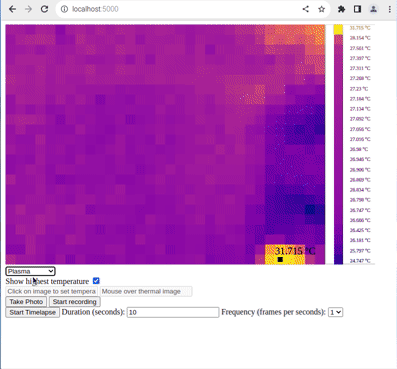
\includegraphics[width=0.8\textwidth]{frame_014_delay-0.1s.png}
  \caption{Interfejs użytkownika}
  \label{fig:obrazek}
\end{figure}









% TODO
\chapter{Uruchomienie}
\label{ch:Uruchomienie}
\section{Dla prowadzącego}

Aby aplikacja została uruchomiona w środowisku przygotowanym przez jednego z współtwórców należy:
\begin{itemize}
    \item[1.] Upewnić się o poprawnym zasilaniu Raspberry Pi
    \item[2.] Uruchomić system 
    \item[3.] Upewnić się o wystąpieniu zielonej sygnalizacji przez diodę led, na module kamery, potwierdzające poprawne podłączenie jej do zasilania.
    \item[4.] Upewnić się o poprawnym połączeniu z modułem poprzez polecenie:\newline \lstinline|$sudo i2cdetect -y 1|.
(  Jeżeli wystąpi problem z uruchomieniem polecenia należy doinstalować brakującą bibliotekę poleceniem: \newline \lstinline|$sudo apt-get install i2c-tools|. )
Poprawna komunikacja Raspberry z kamerą przez interfejs i2c potwierdza wystąpienie liczby 33 w tablicy wypisanej w konsoli.
    \item[5.] W terminalu należy wywołać wówczas za pomoca polecenia python program z sciezka o ile nie znajdujemy sie w jego lokalizacji. Przykładowe polecenie może wyglądać: \lstinline| $python3 Desktop\Framer\framer.py|


\end{itemize}


Aby aplikacja została uruchomiona w nowym środowisku tj Raspberry z kamerą MLX90640, wystarczające powinno być skopiowanie repozytorium pod adresem \lstinline|github.com/michalubczynski/Framer|. W przypadku braku dostępu do sieci, niezbędne biblioteki to kolejno:
\begin{itemize}
\item adafruit-circuitpython-mlx90640
\item flask
\item python-socketio
\end{itemize}
W przypadku braku dostępu do repozytorium lecz posiadając dostęp do sieci, należy wprowadzić w terminalu następujące polecenia:
\newline
\lstinline|pip install adafruit-circuitpython-mlx90640 flask python-socketio|
\newline
\lstinline|python3 framer.py|


\section{Dla uczestnika}

Dostęp do aplikacji uzyskujemy poprzez wprowadzenie w przeglądarce "adresIpAparatu:5000" np: 192.168.0.11:5000 co jest kolejno adresem ip aparatu 192.168.0.11, o ktory należy zapytać operatora, oraz stały port 5000 na ktorym hostowana jest aplikacja. Jeśli na Twojej sieci lokalnej działa firewall, upewnij się, że nie blokuje dostępu do portów, które są używane przez serwer WWW. W przypadku braku dostępu do aplikacji po zapewnieniu poprzednio wspomnianych wymagań, należy skontaktować się z administratorem.
Testowane przeglądarki dostępne dla użytkowników aplikacji:
\begin{itemize}
\item Opera v106.0.4998.2	
\item Opera gx v105.0.4970.37
\item Google Chrome v119.0.6045.209
\item Mozilla Firefox v120.0.1
\item Microsoft Edge v120.0.2210.61
\item Safari v17.1
\item Brave v1.60.125
\item Microsoft Edge v120.0.2210.61
\end{itemize}


% TODO
\chapter{Funkcjonalności}
\label{funkcjonalnosci}

\section {Obraz}
Wyświetlany obraz ma format 32x24 zgodnie z matrycą i jest skalowany na obiekt Canvas o wymiarach 640x480 co daje nam powiększenie rzędu 2000\%. Obraz jest odświeżany dwa razy na sekundę tj. z częstotliwością 2Hz.
\section{Skala temperatury} 
Skala występujących temperatur na obrazie, znajduję się po prawej stronie od obrazu. Posiada dokładnie 24 wartości, najwyższą u góry, najniższą u dołu. Wypisane temperatury odpowiadają kolorowi przy jakim zostały wypisane oraz w jakim kolorze zostały napisane (kolor cyfr odpowiada kolorowi do którego się odnoszą). Tekst posiada czarną obwódkę dla zwiększenia czytelności tekstu. Skala jest dopisywana do zdjęcia o którym mowa w podpunkcie 3.7.
\section{Kolor mapy}
Wyświetlany obraz jest widoczny w jednym dostępnych map kolorów. Oznacza to, że użytkownik w zależności od indywidualnych preferencji, może wybrać dla siebie najbardziej czytelny zestaw wyświetlanych kolorów. Dostępne zestawy to następująco:
\begin{itemize}
    \item \textbf{Inferno}
    
    \begin{figure}[H]
        \centering
        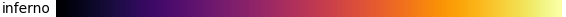
\includegraphics[width=0.8\textwidth]{../../images/Inferno.png}
        \caption{Colormap inferno}
        \label{fig:inferno}
    \end{figure}

    \item \textbf{Plasma}
    
    \begin{figure}[H]
        \centering
        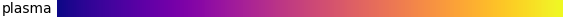
\includegraphics[width=0.8\textwidth]{../../images/Plasma.png}
        \caption{Colormap plasma}
        \label{fig:plasma}
    \end{figure}

    \item \textbf{Rainbow}
    
    \begin{figure}[H]
        \centering
        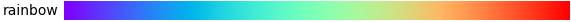
\includegraphics[width=0.8\textwidth]{../../images/Rainbow.png}
        \caption{Colormap rainbow}
        \label{fig:rainbow}
    \end{figure}

    \item \textbf{Seismic}
    
    \begin{figure}[H]
        \centering
        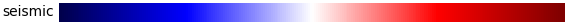
\includegraphics[width=0.8\textwidth]{../../images/Seismic.png}
        \caption{Colormap seismic}
        \label{fig:seismic}
    \end{figure}

    \item \textbf{Greys}
    
    \begin{figure}[H]
        \centering
        
\includegraphics[width=0.8\textwidth]{../../images/Greys.png}
        \caption{Colormap greys}
        \label{fig:greys}
    \end{figure}

    \item \textbf{Hot}
    
    \begin{figure}[H]
        \centering
        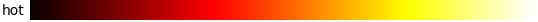
\includegraphics[width=0.8\textwidth]{../../images/Hot.png}
        \caption{Colormap hot}
        \label{fig:hot}
    \end{figure}

    \item \textbf{Hot and Cold}
    
    \begin{figure}[H]
        \centering
        
\includegraphics[width=0.8\textwidth]{../../images/HotAndCold.png}
        \caption{Colormap hot and cold}
        \label{fig:hot-and-cold}
    \end{figure}
\end{itemize}


\section{Najgorętszy punkt na obrazie}
Hot spot to opcja do włączenia, znajdująca się pod obrazem z podpisem "Show highest temperature" która włącza i wyłącza zaznaczanie i wypisywanie najgorętszej temperatury wraz z jej miejscem na obrazie. Do malowania wspomnianego punktu wykorzystywane jest wyznaczanie koloru tła i jego konwersja na biały bądź czarny w zależności który jest bardziej widoczny na tle.
\section{Śledzenie wyznaczonego punktu}
Po kliknięciu na obraz, pojawi się na nim biały punkt którego temperatura jest wypisywana w polu pod obrazem z opisem w zależności od scenariusza. Jeżeli nie został wybrany punkt do śledzenia pojawi się informacja "Click on image to set temperature point". W przeciwnym razie pojawi się "Point position:" z dodaną, aktualizowaną temperaturą punktu który śledzimy.
\section{Śledzenie temperatury pod kursorem}
W czasie rzeczywistym odczytywana jest stale temperatura spod kursora, jeśli kursor znajduje się na wyświetlanym obrazie z kamery, Wówczas temperatura wyświetlana jest jako "Mouse position: ( temperatura *C)". W przeciwnym razie użytkownik jest powiadamiany o wyjechaniu kursorem poza obraz informacją "Mouse over thermal image". Informacje te znajdują się w kontrolce pod obrazem a po lewej stronie od kontrolki z punktu 3.5.
\section{Robienie zdjęć}
Do funkcji robienia zdjęć służy przycisk umiejscowiony pod obrazem, opisany "Take Photo". W momencie jego przyciśnięcia, zostaje pobierany lokalnie przez klienta obraz, wraz ze skalą oraz każdym wskaźnikiem namalowanym na obrazie. Zdjęcie to posiada format .png oraz jest opisane jako \lstinline|thermalImage<dzien_miesiac_rok@godzina_minuta_sekunda.png> |czasu UTC. Obraz ma wymiary 740x480 i jego rozmiar nie powinien przekraczać 50kB. Domyślnym folderem zapisywania jest folder \lstinline|C:\\Downloads |.
\section{Nagrywanie wideo}
Do funkcji nagrywania wideo służy przycisk Start/Stop recording. Jest to przycisk rotacyjny co oznacza, że przy pierwszym wyzwoleniu jest widoczny napis Start recording a przy drugim Stop recording. Takie zachowanie jest naturalne ze względu na możliwości użytkownika do uruchamiania i zatrzymywania nagrywania w dowolnym momencie. Maksymalny czas nagrania został ustawiony na 10 minut po którym w przypadku braku akcji ze strony użytkownika samoistnie zakończy się nagranie i zostanie pobrane lokalnie do folderu \lstinline|C:\\Downloads |. Wideo to posiada format .mp4 oraz jest opisane jako \lstinline|thermalVideo<dzien_miesiac_rok@godzina_minuta_sekunda.png> |czasu UTC. Nagrywanie jest przechwytywane w maksymalnym dostępnym odczycie dwie klatki na sekundę. Podczas nagrywania nie jest dostępna żadna inna funkcja przechwytywania obrazu czyt. robienie zdjęć oraz Timelapse.
\section{Timelapse}
Do funkcji Timelapse służy przycisk Start Timelapse. Do ustawiania czasu trwania timelapse służy pole opisane "Duration" i jest ono opisane w sekundach. W odróżninieniu od wideo, możemu tutaj zmienić ilość klatek na sekundę w celu zaoszczędzenia miejsca na dysku. Dostępne pola to 1 oraz 2 fps. Po zakończeniu czasu trwania timelapse, wideo zostanie pobrane lokalnie do folderu \lstinline|C:\\Downloads |. Wideo to posiada format .mp4 oraz jest opisane jako \lstinline|thermalVideo<dzien_miesiac_rok@godzina_minuta_sekunda.png> |czasu UTC. Uruchomiony Timelapse nie może zostać przerwany w konwencjonalny sposób, lecz może zostać przerwane poprzez odświeżenie przeglądarki.

% TODO
\chapter{Proces rozwoju aplikacji}
\label{proces-rozwoju-aplikacji}
\section{Wybór środowiska i narzędzi}

Wybór środowiska i narzędzi w projekcie Framer.py wynikał z potrzeby stworzenia aplikacji do wizualizacji danych z kamery termowizyjnej w czasie rzeczywistym, która zapewnia interaktywne i przyjazne dla użytkownika doświadczenie.
\begin{itemize}
\item MLX90640 Thermal Camera i Raspberry Pi 4B 
\\Kamera termowizyjna MLX90640 została wybrana ze względu na jej zdolność do przechwytywania danych temperatury w formacie matrycy. Raspberry Pi 4B została wybrana jako platforma ze względu na jej możliwości, w tym obsługę GPIO i możliwość połączenia z MLX90640 za pośrednictwem magistrali I2C.

 
\item SocketIO
\\SocketIO został wykorzystany do komunikacji w czasie rzeczywistym między serwerem a klientem. Wybór ten umożliwia płynne i natychmiastowe aktualizacje danych termicznych na kanwie HTML, zapewniając użytkownikom interaktywne wrażenia.
\item Adafruit 
\\Biblioteka Adafruit CircuitPython dla MLX90640 została wykorzystana do połączenia z kamerą termowizyjną poprzez magistralę I2C. Biblioteki te ułatwiają integrację i komunikację z czujnikiem, zapewniając dokładne i niezawodne pobieranie danych o temperaturze.
\item Flask
\\Flask, lekki i rozszerzalny framework sieciowy, został wybrany do obsługi interfejsu HTML i interakcji z użytkownikiem. Jego prostota sprawia, że nadaje się do tego projektu, umożliwiając szybkie opracowanie aplikacji internetowej do wyświetlania danych termicznych.
\item HTML i Canvas
\\Element HTML canvas został wykorzystany do renderowania danych termicznych w czasie rzeczywistym. Jego elastyczność i łatwość użycia sprawiają, że jest to odpowiedni wybór do tworzenia dynamicznych wizualizacji w przeglądarce internetowej.
\item Python 
\\ Z racji użytkowania klas udostępnionej biblioteki w pythonie adafruit-circuitpython-mlx90640 zdecydowaliśmy nie multiplikować kodu i wykorzystać sprawne rozwiązanie
\end{itemize}

\section{Napotkane problemy}

\begin{itemize}
\item Ilość klientow
\\Z racji posiadanych środków logistycznie zostały przeprowadzone testy na maksymalnie trzech urządzeniach jednocześnie. W razie problemów z większą ilością użytkowników, proszony jest natychmiastowy kontakt z jednym z współtwórców aplikacji.
\item Odswiezanie obrazu
 Częstotliwość odświeżania zadeklarowana przez producenta 0,5 Hz do 64 Hz po przeprowadzonych testach została zdementowana albowiem wartosci powyzej 2Hz wpływały wyłącznie negatywnie na czas odświeżania klatek.
\item UDP a nie TCP
Istnieją przesłanki iż wykorzystywany podczas projektu system dostarczania pakietów TCP nieznacznie spowalnia wyświetlanie obrazu lecz implementacja systemu UDP w sposób znaczący opóźniłaby dostarczenie gotowego produktu. Jest to jeden z problemów do poruszenia w przypadku rozwijania aplikacji.
\item Interpolacja obrazu a wypelnionej canvy
Dodanie obrazu z pliku pozwala używać gotowych implementacji interpolacji, które są zoptymalizowane pod kątem efektywności i jakości. Z racji iż obraz nie jest gotowym obrazem z rozszerzeniem .png a w naszym przypadku jest w każdej iteracji wypełniany kolorami piksel po pikselu, interpolacja musiałaby zostać wykonana własnoręcznie poprzez stworzenie odpowiedniej funkcji. Kod aplikacji zawiera już odpowiednio przygotowaną metodę lecz nie została ona w obecnej wersji przetestowana i zaimplementowana pod obecne warunki środowiska.
\item Zrzuty ekranu i gify
Jednym z problemów które napotkano podczas próby dokumentacji poczyniań był problem z przechwytywaniem ekranu. Instalacja oprogramowania jak: "peek" oraz "byzanz" i wielorazowe próby przechwycenia interfejsu użytkownika, kończyły się zapisem do pliku wyłącznie czarnego koloru. Choć wszystkie ustawienia aplikacji działały i możliwość zmiany czasu nagrywania, rozdzielczości, kompresji czy też pola które będzie przchwytywane, żadno z powyższych nie wpływało na rezultat co zawiera nagranie. Instalacja oprogramowania "simplescreenrecorder" przy uruchamianiu aplikacji, jako pierwsze nakierowało na problem, wyświetlając komunikat o treści braku wsparcia dla sesji z systemem Wayland cyt. :"You are using a non-X11 window system (e.g. Wayland) which is currently not supported". Zapoznając się z dokumentacją oprogramowań które do tej pory zastosowano zaobserwowano trend w tego typu aplikacjach do wsparcia bazowo systemów opartych na X11. Wykorzystując kolejno:
\begin{itemize}
\item \lstinline|$sudo raspi-conifg|\\
\begin{itemize}
	\item Advanced Options-> Wayland-> W1 x11 ( Openbox window manager with X11 backend)\\
Zamiast dotychczas
	\item Advanced Options-> Wayland-> W2 Wayfire ( Wayfire window manager with manager with Wayland backend)
\end{itemize}
\item \lstinline|$ reboot|
 \item \lstinline|$ echo $XDG_CURRENT_DESKTOP|\\
  \lstinline| LXDE|
 \item \lstinline|$ echo $XDG_SESSION_TYPE |\\
  \lstinline| x11|\\
Wówczas każdy z poprzednich edytorów zaczął prawidłowo nagrywać
\end{itemize}
\item Biblioteka do zapisu wideo i kodeki
Początek problemu leżał już w znalezieniu odpowiedniej biblioteki, gdyż ffmeg która była zalecana przez społeczność, nie posiadała odpowiednich dla projektu build'ów. Co za tym idzie kod wcześniej przygotowany wykorzystujący ją, musiał zostać zmodernizowany gdyż sieciowa wersja plików źródłowych nie miała by prawa działania lokalnie bez internetu a lokalnie nie można jej było pobrać z racji praw autorskich. Sama implementacja tej biblioteki także budziła kontrowersje w zespole przez co zdecydowaliśmy się ją odsunąć i zastosować MediaStream recording API która bazowo zapisuje w formacje webm. Według samego producenta posiada ona wsparcie dla rozszerzenie .mp4 oraz kodeków h264 lecz po ich przypisaniu w inicjacji instancji, program się nie uruchamiał. Ku zdziwieniu ustawienia sprzeczne sobie tj inicjacja za pomoca webm a następnie przypisanie zmiennej rozszerzenia .mp4 oraz bazowe kodeki  dla webm działają prawidłowo i obraz jest zapisywany zgodnie z oczekiwaniami.
\end{itemize}


\section{Kontakt i osoby odpowiedzialne}
\begin{itemize}
\item Budowa hardware, instalacja software, logika aplikacji - Michał Lubczyński: michlub322@student.polsl.pl
\item Szata graficzna strony WWW - Andrzej Zagórski: andrzag533@student.polsl.pl
\item Wykorzystane biblioteki, uruchomienie aplikacji - Eryk Szmyt: erykszm832@student.polsl.pl
\end{itemize}


% TODO
\chapter{Podsumowanie i wnioski}

Praca nad aplikacją Framer.py była  wyzwaniem, które pozwoliło na zdobycie doświadczenia w zakresie programowania aplikacji internetowych oraz integracji sprzętu z oprogramowaniem. Projekt umożliwił zastosowanie różnorodnych technologii i narzędzi, takich jak SocketIO, Flask, Adafruit, czy HTML Canvas, w celu stworzenia interaktywnej aplikacji do wizualizacji danych z kamery termowizyjnej MLX90640.\\
Projekt Framer.py jest udanym przykładem zastosowania technologii webowych do wizualizacji danych w czasie rzeczywistym. Praca nad projektem pozwoliła na zdobycie praktycznych umiejętności w obszarze programowania w języku Python, korzystania z różnych bibliotek i frameworków, oraz rozwiązywania problemów związanych z integracją sprzętu i oprogramowania.\\
Aplikacja Framer.py stanowi solidną podstawę do dalszego rozwoju. W przyszłości można by rozważyć dodanie nowych funkcjonalności, takich jak obsługa większej liczby klientów, poprawa algorytmów interpolacji obrazu, czy rozwinięcie opcji nagrywania wideo. Istotnym aspektem jest również dostosowanie aplikacji do różnych platform i systemów operacyjnych oraz testowanie jej działania w różnych środowiskach.\\
Ostatecznie, praca nad projektem Framer.py była wartościowym doświadczeniem, umożliwiającym zdobycie nowych umiejętności i pogłębienie wiedzy w obszarze programowania aplikacji internetowych i integracji sprzętu z oprogramowaniem.






\end{document}




